\thispagestyle{empty}
\section*{Preface I}
\label{sec:prolog_1}

The following thesis was created during the seventh and last semester at the Georg Simon Ohm University of Applied Science. 
Within the last three semesters, I realized that my major interest among all IT related topics is artificial intelligence.

My personal interest started basically with a group IT-project, in which my team and I programmed an autonomously driving remote control car with a deep neural network together with a Raspberry Pi 3B+. From this first project on, I selected all my further elective courses to be related to machine learning or data science in any possible way. I wanted to increase my knowledge further, so I searched for a website that provides courses related to AI. I found \textit{www.udacity.com}, which offers courses in cooperation with top IT companies, such as Google, Airbnb, or Microsoft. Out of curiosity, I bought the course \textit{Natural Language Processing}. After successfully finishing it, I was encouraged to write my bachelor thesis in a \textit{Natural Language Processing} related topic. 
Together with my professor \textit{Prof. Dr. Alfred Holl}, I worked out a method-matrix for the entire structure of this paper. Without his cooperative support overseas while I was studying abroad at the City University of Hong Kong, this thesis would not have been possible for me.
Even though Natural Language Processing is just a subfield of machine learning, the current state-of-the-art research is far beyond what I can research within a bachelor thesis. In this way, I decided to write my thesis about the subfield \textit{textgeneration} within NLP. My state-of-the-art research includes all \textit{hot topics} within NLP, and my prototype focuses only on the text generation part, to dive deeper into what NLP and especially text generation can accomplish in the year 2020.
\null\newpage

\section*{Preface Il}
\label{sec:prolog_2}
For my research, I encountered a lot of old and recently published papers, mostly from \textit{https://arxiv.org/}. 
To read through the papers requires a lot of prior knowledge, especially in mathematics, which I learned in my abroad semester in Hong Kong. 
To fully understand the mathematics given in this thesis, enhanced knowledge of calculus and linear algebra is required. Even if this is not the case, I will describe the process in such a way that it can be comprehended without looking at the maths. \\
Machine Learning and, more specifically, NLP is not an intuitive study. I provided for the matrix notations the common terminologies originated from top researchers and tried to make the entry into this field as smooth as possible if the reader has no prior knowledge about this topic.
During the five-month development process of the bachelor thesis, I gained much knowledge. I recognized that NLP is a huge topic, constantly under research. To keep up to date with the latest publications requires much effort. \\
To give a full state-of-the-art review about \textit{all} NLP related disciplines is not possible within this thesis. For this reason, I focus entirely on the development of the \textit{Neural Text Generation} (NTP), which includes more fields than the reader might imagine.


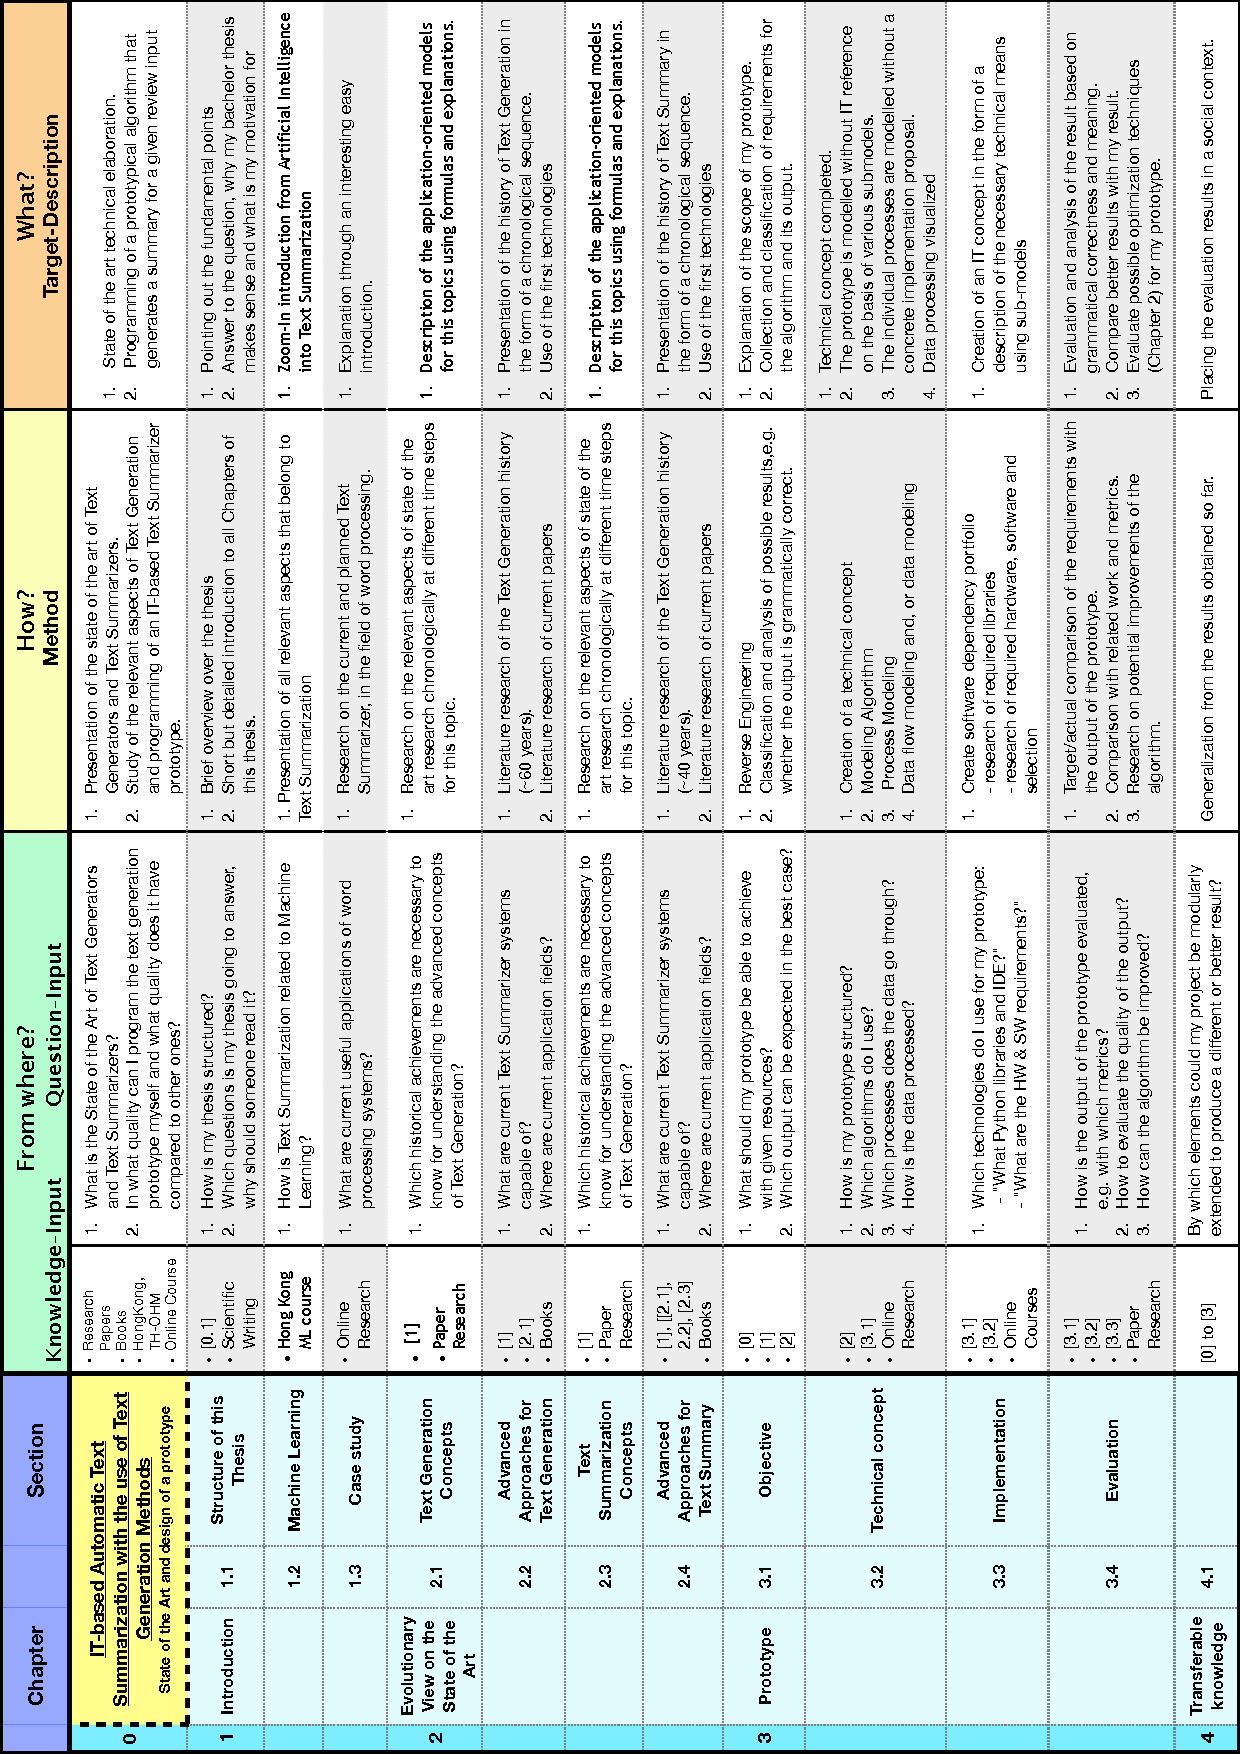
\includepdf[fitpaper=true, pages=-]{methoden_matrix.pdf}

\section*{Abstract}
\label{sec:abstract}

-- At the end , finally finished :) --